\documentclass[10pt,draftclsnofoot,onecolumn,journal,compsoc]{IEEEtran}
% for IEEEtran usage, see http://www.texdoc.net/texmf-dist/doc/latex/IEEEtran/IEEEtran_HOWTO.pdf

\usepackage[margin=0.75in]{geometry}
\usepackage{graphicx}
\usepackage{caption}
\usepackage{hyperref}
\usepackage{enumerate}
\usepackage[dvipsnames]{xcolor}
\usepackage{amssymb}
\usepackage{listings}
\usepackage{float}
\title{A Comparison of Linux, FreeBSD, and Windows}
\author{
  \IEEEauthorblockN{Heidi Clayton} \\
  \IEEEauthorblockA{CS 444: Operating Systems II Spring 2017 \\ Oregon State University}
}

\lstdefinestyle{C_listing}{
  language=C,
  keywordstyle=\color{Fuchsia},
  commentstyle=\itshape\color{ForestGreen},
}
\lstset{style=C_listing}


   
\begin{document}
\maketitle
\newpage
\tableofcontents
\newpage

\section{Introduction}
There are many concepts in the implementation of operating systems and no two operating systems interpret and implement those concepts the same way. In this essay, Linux, FreeBSD, and Windows will be compared on the topics of processes, threads, CPU scheduling, I/O scheduling, memory management, and interrupts.

\section{Processes}
Processes are, at the basic level, instances of some running program. Discussed below are some similarities and differences between different implementations.

\subsection{Linux}
Linux processes are kept in a circular double-linked list of \textit{task\_struct} structures defined in \textit{linux/sched.h}. Each structure is quite large, at around 1.7kb on a 32 bit system. Before the 2.6 kernel version, the \textit{task\_struct} for each process was stored at the end of its stack. This was done so architectures like x86 that have few registers (8 in the case of x86) had a convenient location for the \textit{task\_struct} without having to use a register to store the location. In newer kernels, there is a \textit{thread\_info} structure that has a pointer to the \textit{task\_struct} structure, which is dynamically allocated. It is defined in \textit{asm/thread\_info.h}. This is stored at the beginning or end of the kernel stack, depending on whether the stack grows up or down \cite{linux_proc}.

\begin{lstlisting}[caption={\textit{thread\_info} structure}]
struct thread_info {
        struct task_struct    *task;
        struct exec_domain    *exec_domain;
        unsigned long         flags;
        unsigned long         status;
        __u32                 cpu;
        __s32                 preempt_count;
        mm_segment_t          addr_limit;
        struct restart_block  restart_block;
        unsigned long         previous_esp;
        __u8                  supervisor_stack[0];
};
\end{lstlisting}

The kernel stores a process identification value, or PID, for every process. These can be seen by running the \textit{top} command on the Linux command line, showing running processes and their PIDs. This PID can be used for other commands, like \textit{kill}, as an identifier for the process.

Processes all have a state which determines how the CPU will handle them. The state can be changed using the \textit{set\_current\_state} and \textit{set\_task\_state} functions. A list of possible states is provided in the table below \cite{linux_proc}. \\ \\

\begin{tabular}{ | p{0.45\linewidth} | p{0.45\linewidth} | }
    \hline
    TASK\_RUNNING & The process is either running or in a queue ready to be run. \\ \hline
    TASK\_INTERRUPTIBLE & The process is blocked and waiting for a signal to start running again. \\ \hline
    TASK\_UNINTERRUPTIBLE & The process is blocked but does not wake up at a signal that it is waiting for. \\ \hline
    TASK\_ZOMBIE & The process has finished but its parent has not yet called \textit{wait()}. \\ \hline
    TASK\_STOPPED & The process is not running and not able to run. \\ \hline
\end{tabular} \\ \\ 

Processes are organized in a tree of sorts. The first process is always the \textit{init} process, which has a PID of 1. From then on, processes can be created with the \textit{fork()} function. Each process has a parent, the process it spawned from, and zero or more children, processes that it has spawned \cite{linux_proc}.

\subsection{FreeBSD}
Processes in FreeBSD are represented by the \textit{proc} structure that contains all vital information on the process, such as the PID, flags, and open files. Like Linux, FreeBSD keeps processes in a linked list of dynamically allocated \textit{proc} structures \cite{bsd_proc}. 

\begin{lstlisting}[caption={Excerpt from \textit{proc} structure}]
struct  proc {
        struct  proc *p_forw;           /* Doubly-linked run/sleep queue. */
        struct  proc *p_back;
        struct  proc *p_next;           /* Linked list of active procs */
        struct  proc **p_prev;          /*    and zombies. */

        /* substructures: */
        struct  pcred *p_cred;          /* Process owner's identity. */
        struct  filedesc *p_fd;         /* Ptr to open files structure. */
        struct  pstats *p_stats;        /* Accounting/statistics (PROC ONLY). */
        struct  plimit *p_limit;        /* Process limits. */
        struct  vmspace *p_vmspace;     /* Address space. */
        struct  sigacts *p_sigacts;     /* Signal actions, state (PROC ONLY). */

#define p_ucred         p_cred->pc_ucred
#define p_rlimit        p_limit->pl_rlimit

        int     p_flag;                 /* P_* flags. */
        char    p_stat;                 /* S* process status. */
        char    p_pad1[3];

        pid_t   p_pid;           /* Process identifier. */
        struct  proc *p_hash;    /* Hashed based on p_pid for kill+exit+... */
        struct  proc *p_pgrpnxt; /* Pointer to next process in process group. */
        struct  proc *p_pptr;    /* Pointer to process structure of parent. */
        struct  proc *p_osptr;   /* Pointer to older sibling processes. */
        
        ...

\end{lstlisting}

Also like Linux, FreeBSD has a tree-like organization of its processes. The first process is always \textit{init} with a PID of 1, and each process has a parent process and zero or more child processes. FreeBSD also creates new processes with the \textit{fork()} function. \cite{bsd_proc3}.

Processes in FreeBSD also have states similar to Linux. Below is a description of the FreeBSD process states \cite{bsd_proc}.\\ \\

\begin{tabular}{ | p{0.45\linewidth} | p{0.45\linewidth} | }
    \hline
    NEW & The process has just been created. \\ \hline
    NORMAL & The process has enough resources to begin execution. \\ \hline
    RUNNABLE & Part of the NORMAL state. The process preparing for execution. \\ \hline
    SLEEPING & Part of the NORMAL state. The process is waiting for some event to start running. \textit{wait()}. \\ \hline
    STOPPED & Part of the NORMAL state. The process has been stopped by a signal or its parent process until the parent process terminates. \\ \hline
    ZOMBIE & A finished process that has not yet been freed. \\ \hline
\end{tabular} \\ \\ 

Depending on the state of the process, it is placed on one of two queues. A ZOMBIE process is placed on the \textit{zombproc} list. Otherwise, it is placed on the \textit{allproc} list. 

Overall, processes between Linux and FreeBSD are extremely similar. However, since their CPU scheduling is different, process management is quite different, which is a topic that will be covered a bit later.


\subsection{Windows}
Windows processes are represented by a structure called \textit{EPROCESS}, similar to how Linux processes are represented by a \textit{task\_struct} structure. The structure is opaque and undocumented \cite{win_proc}. The \textit{EPROCESS} structure contains pointers to other structures, similar to Linux.

The \textit{EPROCESS} structure has many fields. There are field common to Linux and other operating systems, such as a PID and flags. There are also fields that Linux does not have in its processes, such as a list of devices, a list of threads, an access token that contains security information about the process and a quota block that contains information on memory quotas \cite{win_proc2}. 

Windows processes are created using the \textit{CreateProcess()} function, which takes 10 parameters, as opposed to the POSIX \textit{fork()} function, which takes none. Unlike Linux, creating a new process with \textit{CreateProcess()} does not automatically create a parent-child relationship between processes like creating a new process with \textit{fork()} does \cite{win_proc3}. 

Process states in Windows are fairly similar to Linux, with a few small differences. Shown below are the states of a Windows process \cite{win_proc4}. \\ \\

\begin{tabular}{ | p{0.45\linewidth} | p{0.45\linewidth} | }
    \hline
    Running & The process is running. \\ \hline
    Ready & The process is in a run queue ready to be run. \\ \hline
    Blocked & The process is blocked and ready to continue once it gets a specific signal. \\ \hline
    Suspend & The process is suspended. Typically used when the OS needs more memory for an incoming process or for tasks like debugging. \\ \hline
    New & The process has been created but is not runnable yet. \\ \hline
    Exit & The process is not running and not able to run. \\ \hline
\end{tabular} \\ \\ 

Overall, Windows processes contain much more information that could reasonably be stored somewhere else and not have be initialized every time a new process is created.

\section{Threads}
Threads are paths of execution within processes. Threads are not very different from processes conceptually. They perform the same work a process can do, except they all do not have a separate address space. Processes can have multiple threads sharing the same resources but executing different tasks. 

\subsection{Linux}
Threads in Linux are interesting in that they are almost exactly the same as a process. The only difference between a thread and a process in Linux is the fact that they share the same address space. Threads are implemented as \textit{task\_struct} structures and scheduled the same as a process. Threads in Linux are considered to be a much more light-weight option than creating multiple separate processes, because when a thread is created from a process, nothing is copied since the thread shares everything with all other threads of the process. If any thread calls one of the \textit{exec()} functions, all other threads belonging to the same process are terminated. The POSIX API for threads is found in the \textit{pthread.h} header file \cite{linux_thrd}. 

\subsection{FreeBSD}
Threads in FreeBSD are different from those in Linux because they are treated as a separate entity from a process. Each process has one or more threads which all have their own corresponding kernel thread which has its own kernel stack \cite{bsd_thrd}. Threads are represented by the \textit{thread} structure shown below.

\begin{lstlisting}[caption={Excerpt from \textit{thread} structure}]
struct thread {
	struct mtx	*volatile td_lock; /* replaces sched lock */
	struct proc	*td_proc;	/* (*) Associated process. */
	TAILQ_ENTRY(thread) td_plist;	/* (*) All threads in this proc. */
	TAILQ_ENTRY(thread) td_runq;	/* (t) Run queue. */
	TAILQ_ENTRY(thread) td_slpq;	/* (t) Sleep queue. */
	TAILQ_ENTRY(thread) td_lockq;	/* (t) Lock queue. */
	LIST_ENTRY(thread) td_hash;	/* (d) Hash chain. */
	struct cpuset	*td_cpuset;	/* (t) CPU affinity mask. */
	struct seltd	*td_sel;	/* Select queue/channel. */
	struct sleepqueue *td_sleepqueue; /* (k) Associated sleep queue. */
	struct turnstile *td_turnstile;	/* (k) Associated turnstile. */
	struct rl_q_entry *td_rlqe;	/* (k) Associated range lock entry. */
	struct umtx_q   *td_umtxq;	/* (c?) Link for when we're blocked. */
	struct vm_domain_policy td_vm_dom_policy;	/* (c) current numa domain policy */
	lwpid_t		td_tid;		/* (b) Thread ID. */
	sigqueue_t	td_sigqueue;	/* (c) Sigs arrived, not delivered. */
#define	td_siglist	td_sigqueue.sq_signals
	u_char		td_lend_user_pri; /* (t) Lend user pri. */

\end{lstlisting}

Overall, although processes are very similar between FreeBSD and Linux, threads are quite different. From a simplicity standpoint, I can see why Linux choses to use the same structure for threads and processes. Although, the threading approach in FreeBSD seems more lightweight than the threading in Linux. 

\subsection{Windows}
Unlike Linux, Windows threads are treated as a separate entity from a process. Each process has a list of threads in its structure which Linux processes do not have since threads are hardly distinct from the process they were created from. All processes start out with one thread, which is different from Linux. In terms of the API, it is used very similarly to Linux. Windows' \textit{CreateThread} is synonymous with Linux' \textit{pthread\_create}. Other comparable functions are Windows' \textit{ThreadExit} and Linux' \textit{pthread\_exit}, and Windows' \textit{WaitForSingleObject} and Linux' \textit{pthread\_join} \cite{win_thrd}. Each thread is represented by an \textit{ETHREAD} structure which has information such as a pointer to the containing process, an access token, and pending I/O requests. Like FreeBSD and unlike Linux, each thread also contains a pointer to a kernel thread.

My thoughts on the Windows implementation are similar to those on the FreeBSD implementation. I think it makes sense to implement threads in a more similar way to their concept as a existing as part of a process.

\section{CPU Scheduling}
CPU scheduling is a vital part of an operating system and varies widely between implementations. CPU scheduling manages running processes. Different scheduling algorithms are used for different needs. 

\subsection{Linux}
In the Linux kernel version 2.6, the scheduler known as the O(1) scheduler was used by default, its namesake being that it takes constant time to schedule a task. Prior to this, the default scheduler ran on O(N) time. The way this scheduler works is by having two arrays of processes; one referred to as the active array and the other referred to as the expired array. The scheduler allocates a fixed quantum to each process in the active array and moves each process to the expired array when the given process has finished its quantum. Then the arrays are switched and the process repeats. The O(1) scheduler gives priority to tasks that it views as being interactive with the user, but the algorithm for computing the amount of interactivity has been criticized as being inaccurate \cite{linux_shd}.

Shortly following the creation of the O(1) scheduler, the Completely Fair Scheduler, or CFS, was implemented as the default Linux scheduler in the 2.6.23 kernel release. The CFS is quite a bit different than the O(1) scheduler. As the name implies, the CFS is based on being "fair" to each process. Each process has a niceness value which is used to determine its priority and the size of its quantum. The niceness value of a given process changes as other processes run. Essentially, the CFS gives priority to processes most starved of CPU time (lower niceness values) in the name of fairness, which gets short simple tasks finished quickly and prevents longer-running tasks from starving. The CFS also does not use a simple run queue, but a tree to store processes waiting for execution. The CFS has time complexity of O(log(N)) \cite{linux_shd}.

\subsection{FreeBSD}
FreeBSD has a default scheduler called the ULE scheduler. The ULE scheduler is more similar to Linux' O(1) scheduler than the CFS. Like the O(1) scheduler, the ULE scheduler keeps two queues; one referred to as the current queue and another referred to as the next queue. Processes with higher priorities are put into the current queue and processes with lower priorities are placed into the next queue. When the current queue is empty, the queues switch. This means that long-running tasks will not starve. Priority and quantum size are recalculated every time a process is put back on a queue. Like the O(1) scheduler, tasks that are seen as more interactive are given high priority to maintain fast throughput. Highly interactive tasks are also given the minimum quantum size so the scheduler can quickly determine when an interactive process is no longer so \cite{bsd_shd}.

Overall, the ULE scheduler is not that similar to Linux' current default scheduler, but it is similar to an old version. I do not see any glaring drawbacks to the ULE scheduler or CFS since both account for interactivity, throughput, and starvation. 

\subsection{Windows}
Looking through Microsoft's documentation regarding thread scheduling, one will notice that there is no specific name of a scheduler mentioned. This is because Windows does not have one specific scheduler and instead has scheduling-related code throughout the kernel and is called the kernel's dispatcher \cite{win_shd}. 

Windows has priority levels of 0-31, with a higher value being higher priority. Windows treats all threads with the identical priorities identically and uses a round robin method of assignment. If none of the highest-priority threads are runnable, the next-highest-priority threads are attempted. If this happens and then a higher-priority thread becomes runnable when a lower-priority thread is running, a context switch occurs and the higher-priority thread is run \cite{win_shd2}. 

Overall, scheduling in Windows seems much simpler than scheduling in Linux using the default CFS. Windows also does not have a dedicated scheduler and instead uses what is referred to as the kernel's dispatcher. I also see more of a chance for starvation using Windows' more simplistic method of scheduling.

\section{I/O Schedulers}
I/O schedulers manage devices' request queues. They decide the order of insertion and dispatching, and occasionally merge requests together to reduce the overhead of dispatching multiple separate requests \cite{linux_proc}.

\subsection{Linux}
Character devices are just a stream of data that is read byte-by-byte. Character devices are simple to schedule since they should just go FIFO. For example, a keyboard is a character device. If you type 'bar', you want 'bar' to be input to the screen in that order, not 'rba' or another combination. It is because of this simplicity that character devices do not have a complicated system for management like block devices do, as described below. \cite{linux_proc}

In the Linux kernel 2.4, the default scheduler was the Linus Elevator. This has been widely regarded as a fairly mediocre scheduler, as it can often just turn into a FIFO for long periods due to how it handles requests that are considered 'old'. The Linux kernel 2.6 has three built-in I/O schedulers, the CFQ (Completely Fair Queue) scheduler, the Deadline scheduler, and the No-op scheduler. The CFQ scheduler is similar to the previously discussed CFS, as it tries to schedule I/O 'fairly' to prevent starvation while keeping throughput high. It is the default scheduler and is a good all-purpose scheduler \cite{linux_proc}. 

The Deadline scheduler bases scheduling on each request having an expiration time. The default expiration time for a read request is 500ms and 5s for write requests. There are three queues, a read FIFO, and write FIFO, and a sorted queue that is sorted by disk location. The Deadline scheduler starts by dispatching requests from the head of the sorted queue. Then, if the head of the read or write FIFOs expire, requests start being dispatched from those \cite{linux_proc}. 

The No-op scheduler doesn't do much by design. It simply puts requests in a FIFO. This is ideal for scheduling on devices such as SSDs that already have built-in scheduling where a more complex scheduler like Deadline of CFQ would not be necessary \cite{linux_proc}. 

All of the schedulers' functions are managed by having a structure of function pointers, as shown below.

\begin{lstlisting}[caption={The \textit{elevator\_ops} structure in the linux/elevator.h file}]
struct elevator_ops
{
	elevator_merge_fn *elevator_merge_fn;
	elevator_merged_fn *elevator_merged_fn;
	elevator_merge_req_fn *elevator_merge_req_fn;
	elevator_allow_bio_merge_fn *elevator_allow_bio_merge_fn;
	elevator_allow_rq_merge_fn *elevator_allow_rq_merge_fn;
	elevator_bio_merged_fn *elevator_bio_merged_fn;

	elevator_dispatch_fn *elevator_dispatch_fn;
	elevator_add_req_fn *elevator_add_req_fn;
	elevator_activate_req_fn *elevator_activate_req_fn;
	elevator_deactivate_req_fn *elevator_deactivate_req_fn;

	elevator_completed_req_fn *elevator_completed_req_fn;

	elevator_request_list_fn *elevator_former_req_fn;
	elevator_request_list_fn *elevator_latter_req_fn;

	elevator_init_icq_fn *elevator_init_icq_fn;	/* see iocontext.h */
	elevator_exit_icq_fn *elevator_exit_icq_fn;	/* ditto */

	elevator_set_req_fn *elevator_set_req_fn;
	elevator_put_req_fn *elevator_put_req_fn;

	elevator_may_queue_fn *elevator_may_queue_fn;

	elevator_init_fn *elevator_init_fn;
	elevator_exit_fn *elevator_exit_fn;
	elevator_registered_fn *elevator_registered_fn;
};
\end{lstlisting}

Cryptography in Linux is done with the Crypto API. When a read request is done on an encrypted device, the function \textit{crypto\_cipher\_decrypt\_one} is called. Similarly, when a write request is done on an encrypted device, the function \textit{crypto\_cipher\_encrypt\_one} is called. The API is located in the linux/crypto.h file.

\subsection{FreeBSD}
FreeBSD uses one I/O scheduling method called CAM, or Common Access Method. I/O in FreeBSD is implemented as a stack of sorts. The top half of the stack are things like memory mapped files and a buffer cache, the next part of the stack filters data (including encryption) and includes RAID, and CAM is at the bottom and handles queuing \cite{bsd1}. One interesting thing to note about I/O in FreeBSD is that there is no concept of block devices. Everything is treated as a character device. The CAM scheduler has separate read, write, and delete queues. The CAM scheduler can limit the number of requests in a device at one time as well as have a fairness bias. The fairness bias essentially means that the scheduler "choose[s] one type vs. the other with a predicable bias when the queue has both types in it" when choosing between read and write requests \cite{bsd2}. Figure 1 demonstrates a graph of the workflow done by the CAM scheduler.

A search for information on the CAM scheduler yields many results mentioning NetFlix. This is because NetFlix contributed to the development. With the old FreeBSD I/O scheduler, the read time for I/O requests was much too high on SSDs, as illustrated in Figure 2. \\ \\

\begin{figure}[H]
\centering
    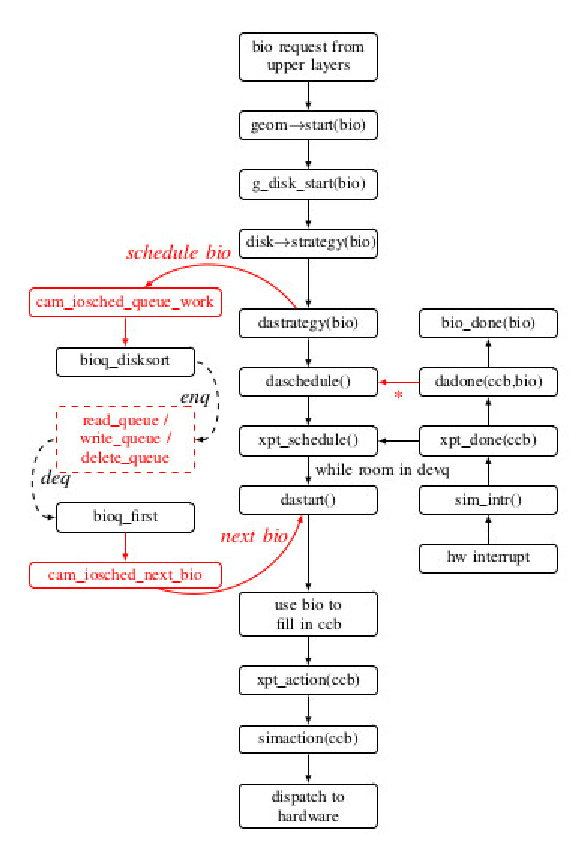
\includegraphics[scale=1.0]{graph2.eps}
    \caption{A graph of the workflow done by the CAM scheduler. The red indicates what is different between CAM and the old default scheduler \cite{bsd2}.}
\end{figure}

\begin{figure}[H]
\centering
    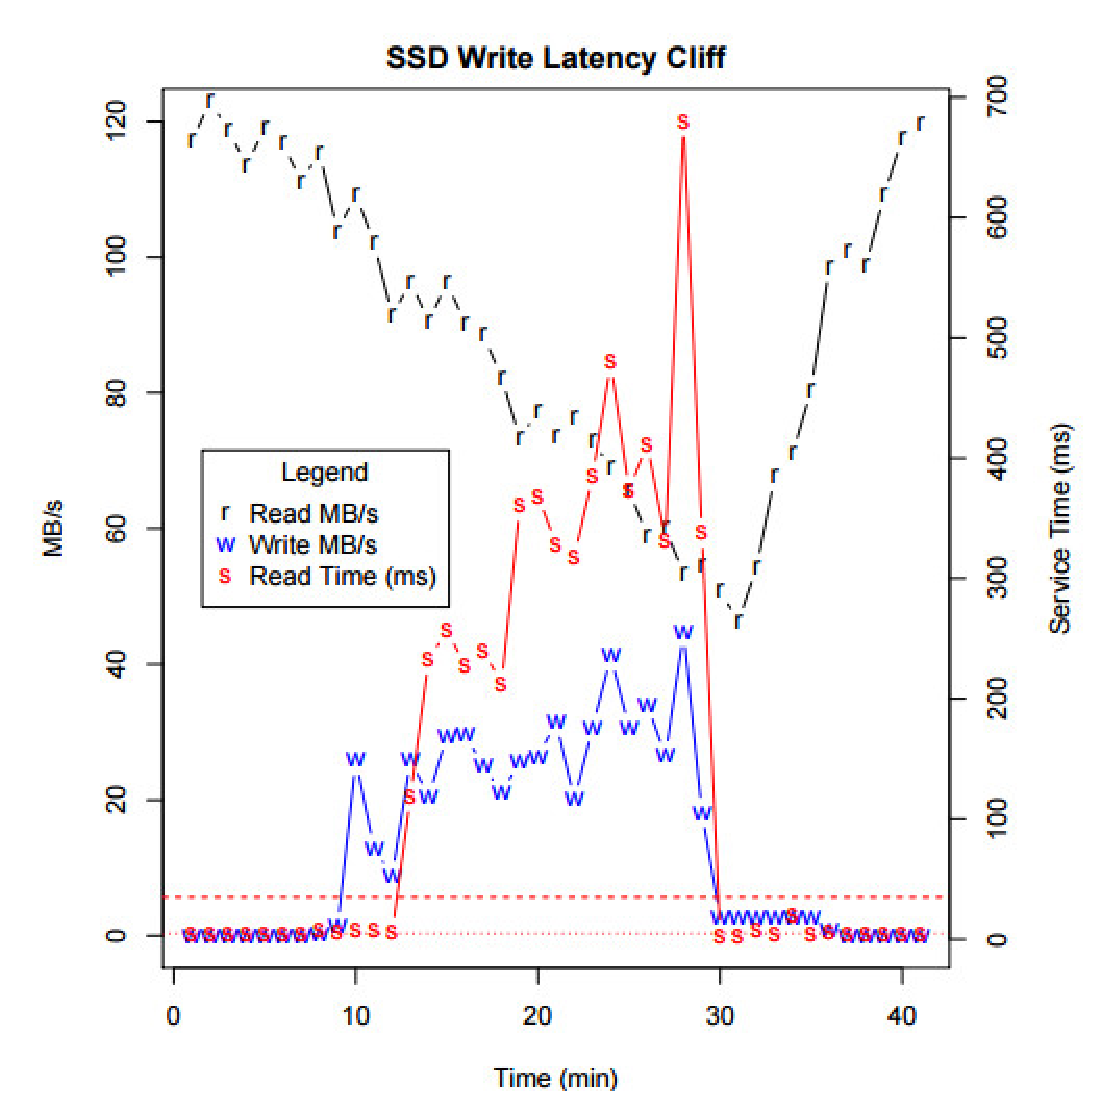
\includegraphics[scale=.6]{graph.eps}
    \caption{A graph of reads and writes done by the old default FreeBSD I/O scheduler. Note that the red line, read time, spikes heavily \cite{bsd2}.}
\end{figure}

\subsection{Windows}
In Windows, the I/O scheduling algorithms are referred to as 'strategies' and are divided into hierarchy prioritization and idle prioritization. There are only 5 priority levels, listen below, and they determine how I/O requests are scheduled \cite{win_shd}. \\ \\
\begin{tabular}{ | p{0.2\linewidth} |}
    \hline
    Critical\\ \hline
    High \\ \hline
    Normal \\ \hline
    Low \\ \hline
    Very low \\ \hline
\end{tabular} \\ \\ 

All requests that are of the 'very low' priority are scheduled via idle prioritization and the rest are scheduled via hierarchy prioritization. The default priority is 'normal'. Applications that do tasks in the background (e.g. Windows Defender) are generally assigned a priority of 'very low'. All requests made by the kernel have at least 'normal' priority, which is a concept called \textit{kernel bump} \cite{win_shd}.

Hierarchy prioritization has a simple underlying concept for scheduling. All 'critical' tasks must be dispatched before 'high' tasks, all 'high' tasks must be dispatched before 'normal' tasks, and all 'normal' tasks must be dispatched before 'low' tasks. Hierarchy prioritization has its own queue \cite{win_shd}.

Idle prioritization has its own queue as well. In general, tasks on the hierarchy prioritization's queue are dispatched first since their priorities are higher. Here, there is a very clear chance for starvation. As long as there is at least one request on the hierarchy prioritization's queue, requests on the idle prioritization's queue will starve. To avoid this, idle prioritization enforces at least one request on its queue is dispatched per unit of time (generally .5s). The ATA and USB port drivers use hierarchy prioritization and SCSI and storage port drivers use idle prioritization \cite{win_shd}. 

Cryptography in Windows can be done with the FileInfo API used with .NET. The methods \textit{Encrypt} and \textit{Decrypt} do what they say on the box \cite{wincrypt}. Entire volumes are encrypted and decrypted using BitLocker, which is included on Windows operating systems starting with Windows Vista \cite{wincrypt2}.

Overall, Windows has less variety when it comes to I/O scheduling algorithms and the scheduling algorithms appear to be fairly simple at a glance.

\section{Memory Management}
\subsection{Linux}
Memory is divided into units called \textit{pages}. Pages are typically 4096 bytes long, however this is not the case for all machines. The size can be found in the \textit{linux/mm.h} file in the \textit{PAGE\_SIZE} constant \cite{linux_proc}. An excerpt of the \textit{page} structure is shown below.
 
\begin{lstlisting}[caption={An excerpt from the \textit{page} structure in the linux/mm.h file.}]
struct page {
	/* First double word block */
	unsigned long flags;		/* Atomic flags, some possibly
					 * updated asynchronously */
	union {
		struct address_space *mapping;	/* If low bit clear, points to
						 * inode address_space, or NULL.
						 * If page mapped as anonymous
						 * memory, low bit is set, and
						 * it points to anon_vma object:
						 * see PAGE_MAPPING_ANON below.
						 */
		void *s_mem;			/* slab first object */
		atomic_t compound_mapcount;	/* first tail page */
		/* page_deferred_list().next	 -- second tail page */
	};

	/* Second double word */
	union {
		pgoff_t index;		/* Our offset within mapping. */
		void *freelist;		/* sl[aou]b first free object */
		/* page_deferred_list().prev	-- second tail page */
	};
\end{lstlisting}
Other notable variables in the \textit{page} structure are \textit{count}, \textit{virtual}, and \textit{flags}. \textit{count} refers to the number of references to the current page. When it hits zero, the page is freed. \textit{virtual} is a pointer to the kernel virtual address of the page. \textit{flags} contains the status of the page set by bits \cite{linux_proc}. 

Not all pages are the same in Linux, however. Pages are broken up into three categories, known as \textit{zones}, which are listed below \cite{linux_proc}. \\

\begin{tabular}{ | p{0.2\linewidth} | p{0.4\linewidth} |}
    \hline
    ZONE\_DMA & Zone containing pages compatible with direct memory access.\\ \hline
    ZONE\_NORMAL & Zone containing normal, mapped pages.\\ \hline
    ZONE\_HIGHMEM & Zone contains pages in high memory, which are not permanently 		mapped into kernel's address space.\\ \hline
\end{tabular} \\ \\ 
Each zone is also represented by a structure appropriately called \textit{zone}, listen below.

\begin{lstlisting}[caption={The \textit{zone} structure in the linux/mmzone.h file.}]
struct zone {
        spinlock_t              lock;
        unsigned long           free_pages;
        unsigned long           pages_min;
        unsigned long           pages_low;
        unsigned long           pages_high;
        unsigned long           protection[MAX_NR_ZONES];
        spinlock_t              lru_lock;
        struct list_head        active_list;
        struct list_head        inactive_list;
        unsigned long           nr_scan_active;
        unsigned long           nr_scan_inactive;
        unsigned long           nr_active;
        unsigned long           nr_inactive;
        int                     all_unreclaimable;
        unsigned long           pages_scanned;
        int                     temp_priority;
        int                     prev_priority;
        struct free_area        free_area[MAX_ORDER];
        wait_queue_head_t       *wait_table;
        unsigned long           wait_table_size;
        unsigned long           wait_table_bits;
        struct per_cpu_pageset  pageset[NR_CPUS];
        struct pglist_data      *zone_pgdat;
        struct page             *zone_mem_map;
        unsigned long           zone_start_pfn;
        char                    *name;
        unsigned long           spanned_pages;
        unsigned long           present_pages;
};
\end{lstlisting}
The function \textit{kmalloc} can be used to allocate memory on the kernel as well as the \textit{vmalloc} function. The difference is that \textit{kmalloc} allocates memory that is physically contiguous while \textit{vmalloc} allocates memory that is virtually contiguous. Another method of memory management is called the SLAB allocator. Basically, the SLAB allocator was designed to have caches of already allocated data structures for common structures such as \textit{inode} and \textit{task\_struct}. This is more efficient than constantly allocating and deallocating memory. Each of these caches is divided into a \textit{slab}, which is typically one page, but can be multiple physically contiguous pages \cite{linux_proc}. The SLAB allocator has queues of slabs per node per CPU, which is a lot of queues. On large systems, those queues can grow exponentially \cite{slub}.  

There is also the SLOB allocator. The SLOB allocator uses a first-fit algorithm which simply finds the first available piece of memory that is large enough for the current data. Because of this simple algorithm, there is often a lot of memory fragmentation. Therefore, it is generally only recommended to be used in embedded systems or in very small systems. 

Finally, there is the SLUB allocator, which is the current default on the Linux kernel. The SLUB allocator is designed to be more scalable than the SLAB allocator. Slabs in SLUB are collections of pages with objects of a given size. The metadata for each slab is also not stored at the top of the slab like it is in the SLAB allocator, making slabs easier to align. Overall, there are also fewer queues than the SLAB allocator \cite{slub}.

\subsection{FreeBSD}
There are 6 layers to how FreeBSD manages the kernel's address space, shown below \cite{bsd_proc}. \\

\begin{tabular}{ | p{0.2\linewidth} | p{0.4\linewidth} |}
    \hline
    Buckets & Per-CPU allocation of objects.\\ \hline
    Zones & Allocation of objects from kegs to buckets.\\ \hline
    Kegs & Collection of slabs of a given object.\\ \hline
    Slabs & Allocation of a set of objects from vmem. \\ \hline
    Vmem & Multiple-of-page allocations from vm\_map.\\ \hline
    Vmem\_map & Address space partitioning. \\ \hline
\end{tabular} \\ \\ 

Like Linux, memory is also divided into pages. Memory on the kernel can be allocated with the function \textit{kmem\_malloc} similar to Linux' \textit{kmalloc} and \textit{vmalloc}. FreeBSD also has a slab memory management system. Each slab is limited to only one page (unless the object needs more than one page). This is to reduce fragmentation. The allocators for the other parts of virtual memory are fairy simple, though there are three different choices for the bottom layer address space partitioning. An allocation request can choose one of the 3 algorithms listed below for memory allocation \cite{bsd_proc}. \\

\begin{tabular}{ | p{0.2\linewidth} | p{0.4\linewidth} |}
    \hline
   VM\_BESTFIT & Finds the smallest segment on the freelist that satisfies the request. \\ \hline
    VM\_INSTANTFIT & If the size of the request is $2^{n}$, take the first segment of freelist[n], otherwise take the first segment of freelist[n + 1].  \\ \hline
    VM\_NEXTFIT & Ignores the freelist and just chooses the next suitable segment after the previous allocation. \\ \hline
\end{tabular} \\ \\ 

The best-fit algorithm is great for reducing fragmentation but can be slow on larger systems. The instant-fit algorithm is the default, as it provides near-constant time performance. The next-fit algorithm is not commonly used and is not supported in all FreeBSD systems though Solaris supports it for allocating process identifiers and the like \cite{bsd_proc}. 

\subsection{Windows}
Kernel memory in Windows is divided into two parts: non-paged pool and paged pool. The non-paged pool part of memory consists of ranges of virtual memory that are also guaranteed to exist in physical memory and can be accessed at any time and therefore by any interrupt request level. The paged pool portion of memory that can be paged in or out of the system. Drivers that do not need to access memory from the dispatch level or above can access paged pool memory and it is also accessible from all process contexts \cite{win_shd}. 

Windows systems start with 4 paged pools and 1 non-paged pools and more are created depending on the number of non-uniform memory access nodes are on the system. The starting size of non-paged pools are 3\% of the system's RAM, or 40MB if 3\% of the system's RAM is less than that and 10\% of RAM is more than 40MB. Otherwise, 10\% of RAM is chosen. The maximum size of an non-paged pool is the smallest of either 75\% of physical memory or 2GB (128GB on 65-bit systems). The maximum size of a paged pool is 2GB on a 32-bit system or 128GB on a 64-bit system \cite{win_shd}. 

Similar to the slab memory allocation on Linux and FreeBSD, Windows has what is called look-aside lists. These lists are made up of pre-allocated blocks of the same size. Lists are created for commonly used structures for each processor. Drivers are allowed to create their own look-aside lists with the functions \textit{ExInitializeNPagedLookasideList} for non-paged pools and \textit{ExInitializePagedLookasideList}. Functions similar to Linux' \textit{kmalloc} and \textit{vmalloc} and FreeBSD's  \textit{kmem\_malloc} are \textit{HeapAlloc}, \textit{HeapCreate}, and \textit{HeapRealloc} \cite{win_shd}. 

\section{Interrupts}
Interrupts are a crucial part of communication between the hardware and processor. For example, the keyboard controller sends out a signal to the processor to let the operating system know about the key presses. That signal is what is known as an interrupt \cite{linux_proc}.

\subsection{Linux}
 In Linux, certain types of devices are represented by values that are called Interrupt Requests. For example, a keyboard is represented by the IRQ "one". These IRQs are serviced by what are called interrupt handlers. Interrupt handlers are just basic C functions that follow a standard format, seen in the code below \cite{linux_proc}.
 
\begin{lstlisting}[caption={The \textit{request\_irq} prototype in the linux/interrupt.h file. Note that the \textit{handler} parameter is a function pointer to the interrupt handler.}]
/* request_irq: allocate a given interrupt line */
int request_irq(unsigned int irq,
                irqreturn_t (*handler)(int, void *, struct pt_regs *),
                unsigned long irqflags,
                const char *devname,
                void *dev_id)
\end{lstlisting}
Processing interrupts is broken into two parts. The first part is the aforementioned interrupt handler, referred to as a "top half". Interrupt handlers are written with just the basics in mind. They perform any crucial operations, such as resetting the hardware. The other part of the process is called a "bottom half". Bottom halves do the rest of the work that isn't time-critical, such as processing packets from network cards \cite{linux_proc}. 

Bottom halves are a bit different in implementation from top halves. Top halves only have one exact way they can be written, but bottom halves have three. The three different types of bottom halves are known as softirqs, tasklets, and work queues. What one is ideal to be used depends on the type of work that needs to be done. 

Softirqs are generally pretty good to use for tasks that require many threads. They never pre-empt each other and the same softirq can be run on multiple CPUs at the same time. They are also the least used in the Linux kernel and for a few reasons. One is that they are statically allocated, so they cannot be destroyed or dynamically created. Another is that the kernel has a limit of only 32 softirqs allowed to exist at once, which are stored in an array in kernel/softirq.c called \textit{softirq\_vec} \cite{linux_proc}. Each entry in this array is of the structure type listed below.
\begin{lstlisting}[caption={The \textit{softirq\_action} structure in the linux/interrupt.h file.}]
/*
 * structure representing a single softirq entry
 */
struct softirq_action {
        void (*action)(struct softirq_action *); /* function to run */
        void *data;                              /* data to pass to function */
};
\end{lstlisting}
Softirqs are given a priority and are scheduled via that priority. Below is a list of important softirq priorities \cite{linux_proc}. They can be found in linux/interrupt.h. \\ \\
\begin{tabular}{ | p{0.25\linewidth} | p{0.25\linewidth} | p{0.25\linewidth} | }
    \hline
Tasklet & Priority & Description \\ \hline
HI\_SOFTIRQ & 0 & High-priority tasklets \\ \hline
TIMER\_SOFTIRQ & 1 & Timer bottom half \\ \hline
BLOCK\_SOFTIRQ & 4 & Block devices \\ \hline
TASKLET\_SOFTIRQ & 5 & Tasklets \\ \hline
SCHED\_SOFTIRQ & 6 & Scheduler \\ \hline
\end{tabular} \\ \\ 
Tasklets are built on top of softirqs are are the most used. Tasklets can be dynamically allocated and destroyed and one tasklet can only be run on one CPU at once. Below is the structure for a tasklet.

\begin{lstlisting}[caption={The \textit{tasklet\_struct} structure in the linux/interrupt.h file.}]
struct tasklet_struct {
        struct tasklet_struct *next;  /* next tasklet in the list */
        unsigned long state;          /* state of the tasklet */
        atomic_t count;               /* reference counter */
        void (*func)(unsigned long);  /* tasklet handler function */
        unsigned long data;           /* argument to the tasklet function */
};
\end{lstlisting}
Tasklets are also run based on priority values. They are scheduled with either the \textit{HI\_SOFTIRQ} or \textit{TASKLET\_SOFTIRQ} priorities. 

Work queues are quite different than softirqs and tasklets. While softirqs and tasklets are run in the interrupt context, work queues are run in the process context. This means that they can be scheduled and sleep just like a normal process. If work needs to be able to sleep, work queues are the ideal option. Otherwise, use a tasklet. The structure of a work queue is found below.

\begin{lstlisting}[caption={The \textit{workqueue\_struct} structure in the linux/workqueue.h file.}]
/*
 * The externally visible workqueue abstraction is an array of
 * per-CPU workqueues:
 */
struct workqueue_struct {
        struct cpu_workqueue_struct cpu_wq[NR_CPUS];
        const char *name;
        struct list_head list;
};
\end{lstlisting}

\subsection{FreeBSD}
Like Linux, FreeBSD also has a concept of top and bottom halves when processing interrupt requests. FreeBSD has three types of interrupts. There are driver interrupts, software interrupts, and clock interrupts. 

Driver interrupts are similar to threads in FreeBSD. Interrupts are run in the process context and cannot access the context of any previously processed interrupts. They also have their own stack. Like Linux work queues, these types of interrupts can sleep \cite{bsd_proc}. 

Software interrupts are scheduled at a lower priority than driver interrupts. They too are run in the process context and can block. When interrupts are scheduled, driver interrupts go first. When there are no more of them, the next software interrupt goes next. If a higher-priority interrupt request happens while a software interrupt is being processed, it is pre-empted and the higher-priority interrupt request is processed \cite{bsd_proc}.

Clock interrupts are quite different from driver and software interrupts. Clock interrupts are referred to as \textit{ticks} and happen 1000 times per second. This is done so that the system's time is updated as well as user-process and system timers. These interrupts are scheduled at a very high priority. There are not many situations where it will be waiting on another interrupt \cite{bsd_proc}.  

\subsection{Windows}
In Windows, when an interrupt request is triggered, the kernel saves the state of the processor and then resumes that state when the interrupt request is done being processed. The kernel then queries the interrupt controller (usually a variant of the i82489 Programmable Interrupt Controller on x86 systems) which then assigns a number to the interrupt request, similar to Linux requests. This number is used to insert the interrupt into a table known as the Interrupt Dispatch Table, or IDT. When Windows boots, the elements of the IDT are assigned pointers to the appropriate routines to handle them \cite{win_shd}. 

Software requests, though less common than hardware interrupts, have an important place on the Windows operating system. Types of tasks that that are facilitated by software interrupts are thread dispatching, asynchronous I/O, and timer expiration, among others. One specific type of software interrupt is called a Dispatch or Deferred Procedure Call, or DPC. These types of software interrupts are enacted when a thread is sleeping or has terminated. The interrupt request is send in order to facilitate a context switch, as discussed in the CPU scheduling section \cite{win_shd}.

Windows also has priority levels for interrupts. They range from 0 to 31 on x86 systems. Unlike Linux, a higher number means higher priority. Generally, hardware interrupts have priorities ranging from 3 to 31 and software interrupts have priorities of 2 or 1 \cite{win_shd}. 

\section{Conclusion}
As you can see, Linux, FreeBSD, and Windows all have their differences in the implementations of their operating systems. FreeBSD and Linux tend to be a bit more similar, which makes sense as they are both Unix-like operating systems. Windows, while still having its differences such as not having a dedicated CPU scheduler, is still similar in many ways such as Windows' threads' similarities to FreeBSD's threads. Overall, operating systems tend to take similar concepts and implement them a little differently than their predecessors. 

\newpage

\begin{thebibliography}{18}

\bibitem{linux_proc}
Love, R. \textit{Linux Kernel Development}. 2nd ed. Indianapolis, IN: Novell, 2005. Print. \\
Available: \url{http://www.makelinux.net/books/lkd2/ch03lev1sec1}

\bibitem{win_proc}
"EPROCESS." Windows Drivers. Microsoft, n.d. Web. 01 May 2017. \\
Available: \url{https://msdn.microsoft.com/en-us/library/windows/hardware/ff544273(v=vs.85).aspx}

\bibitem{win_proc2}
Russinovich, M., and D. A. Solomon. "Processes, Threads, and Jobs in the Windows Operating System." \textit{The Microsoft Press Store}. Pearson Education, 17 June 2009. Web. 01 May 2017. \\
Available: \url{https://www.microsoftpressstore.com/articles/article.aspx?p=2233328}

\bibitem{win_proc3}
"Processes in Unix, Linux, and Windows." Worcester Polytechnic Institute, 2008. Web. 1 May 2017. \\
Available: \url{https://web.cs.wpi.edu/~cs3013/c08/LectureNotes--c08/Week\%202,\%20Linux-Windows\%20Processes.ppt}

\bibitem{win_proc4}
"Windows Process and Threads: C Run-Time 6 | Main | Windows Process and Threads Programming." \textit{The Tenouk's C, C++, Linux and Windows Network, Win32, Winsock/socket, STL, Windows GUI/MFC Programming Tutorials}. Tenouk, n.d. Web. 01 May 2017. \\
\url{http://www.tenouk.com/ModuleT.html}

\bibitem{bsd_proc}
McKusick, M. K., G. V. Neville-Neil, and R. N. M. Watson. \textit{The Design and Implementation of the FreeBSD Operating System}. Upper Saddle River: Addison-Wesley/Pearson, 2015. Print.

\bibitem{bsd_proc3}
"Chapter 3. FreeBSD Basics." \textit{FreeBSD}. FreeBSD, n.d. Web. 01 May 2017. \\
Available: \url{https://www.freebsd.org/doc/handbook/basics-processes.html}

\bibitem{linux_thrd}
Mitchell, M., J. Oldham, and A. Samuel. \textit{Advanced Linux Programming}. Indianapolis, Ind. ; Munich: New Riders, 2003. Print. \\
Available: \url{http://advancedlinuxprogramming.com/alp-folder/}

\bibitem{bsd_thrd}
"A Look Inside." \textit{FreeBSD}. FreeBSD, n.d. Web. 01 May 2017. \\

\bibitem{win_thrd}
"Processes and Threads." System Services. Microsoft, n.d. Web. 01 May 2017. \\
Available: \url{https://msdn.microsoft.com/en-us/library/windows/desktop/ms684847(v=vs.85).aspx}

\bibitem{win_thrd2}
Russinovich, M. E., and D. A. Solomon. "Processes, Threads, and Jobs in the Windows Operating System." \textit{Microsoft Press Store}. Pearson Education, 06 June 2009. Web. 01 May 2017. \\
Available: \url{https://www.microsoftpressstore.com/articles/article.aspx?p=2233328&seqNum=4}

\bibitem{linux_shd}
Pabla, C. S. "Completely Fair Scheduler." \textit{Linux Journal}. Linux Journal, 01 Aug. 2009. Web. 01 May 2017. \\
Available: \url{http://www.linuxjournal.com/magazine/completely-fair-scheduler}

\bibitem{bsd_shd}
Roberson J. ULE: A Modern Scheduler for FreeBSD. In BSDCon 08 Sept. 2003. (pp. 17-28). \\
Available: \url{http://web.cs.ucdavis.edu/~roper/ecs150/ULE.pdf}

\bibitem{win_shd}
Russinovich, M. E., D. A. Solomon, and A. Ionescu. \textit{Windows Internals}. Redmond (Wash.): Microsoft, 2012. Print.

\bibitem{win_shd2}
"Scheduling Priorities." System Services. Microsoft, n.d. Web. 01 May 2017. \\
\url{https://msdn.microsoft.com/en-us/library/windows/desktop/ms685100(v=vs.85).aspx}

\bibitem{bsd1}
Losh, W. M. "CAM I/O Scheduler." Warner's Boring FreeBSD Page. FreeBSD, 15 Apr. 2015. Web. 17 May 2017.
Available: \url{https://people.freebsd.org/~imp/asiabsdcon2015/iosched-slides.pdf}

\bibitem{bsd2}
Losh, W. M. "I/O Scheduling in FreeBSD’s CAM Subsystem." Warner's Boring FreeBSD Page. FreeBSD, 2015. Web. 18 May 2017. \\
Available: \url{https://people.freebsd.org/~imp/bsdcan2015/iosched-v3.pdf}

\bibitem{wincrypt}
"FileInfo Methods." .NET Development. Microsoft, n.d. Web. 18 May 2017. \\
Available: \url{https://msdn.microsoft.com/en-us/library/system.io.fileinfo_methods(v=vs.110).aspx}

\bibitem{wincrypt2}
Paul, I. "A Beginner's Guide to BitLocker, Windows' Built-in Encryption Tool." PCWorld. PCWorld, 01 Aug. 2016. Web. 18 May 2017. \\
Available: \url{http://www.pcworld.com/article/2308725/encryption/a-beginners-guide-to-bitlocker-windows-built-in-encryption-tool.html}

\bibitem{slub}
"The SLUB Allocator." \textit{LWN.net}. Eklektix, Inc., 11 Apr. 2007. Web. 05 June 2017. \\
Available: https://lwn.net/Articles/229984/


\end{thebibliography}


\end{document}
